% Options for packages loaded elsewhere
% Options for packages loaded elsewhere
\PassOptionsToPackage{unicode}{hyperref}
\PassOptionsToPackage{hyphens}{url}
\PassOptionsToPackage{dvipsnames,svgnames,x11names}{xcolor}
%
\documentclass[
  11pt,
]{article}
\usepackage{xcolor}
\usepackage[margin=1in]{geometry}
\usepackage{amsmath,amssymb}
\setcounter{secnumdepth}{5}
\usepackage{iftex}
\ifPDFTeX
  \usepackage[T1]{fontenc}
  \usepackage[utf8]{inputenc}
  \usepackage{textcomp} % provide euro and other symbols
\else % if luatex or xetex
  \usepackage{unicode-math} % this also loads fontspec
  \defaultfontfeatures{Scale=MatchLowercase}
  \defaultfontfeatures[\rmfamily]{Ligatures=TeX,Scale=1}
\fi
\usepackage{lmodern}
\ifPDFTeX\else
  % xetex/luatex font selection
\fi
% Use upquote if available, for straight quotes in verbatim environments
\IfFileExists{upquote.sty}{\usepackage{upquote}}{}
\IfFileExists{microtype.sty}{% use microtype if available
  \usepackage[]{microtype}
  \UseMicrotypeSet[protrusion]{basicmath} % disable protrusion for tt fonts
}{}
\makeatletter
\@ifundefined{KOMAClassName}{% if non-KOMA class
  \IfFileExists{parskip.sty}{%
    \usepackage{parskip}
  }{% else
    \setlength{\parindent}{0pt}
    \setlength{\parskip}{6pt plus 2pt minus 1pt}}
}{% if KOMA class
  \KOMAoptions{parskip=half}}
\makeatother
% Make \paragraph and \subparagraph free-standing
\makeatletter
\ifx\paragraph\undefined\else
  \let\oldparagraph\paragraph
  \renewcommand{\paragraph}{
    \@ifstar
      \xxxParagraphStar
      \xxxParagraphNoStar
  }
  \newcommand{\xxxParagraphStar}[1]{\oldparagraph*{#1}\mbox{}}
  \newcommand{\xxxParagraphNoStar}[1]{\oldparagraph{#1}\mbox{}}
\fi
\ifx\subparagraph\undefined\else
  \let\oldsubparagraph\subparagraph
  \renewcommand{\subparagraph}{
    \@ifstar
      \xxxSubParagraphStar
      \xxxSubParagraphNoStar
  }
  \newcommand{\xxxSubParagraphStar}[1]{\oldsubparagraph*{#1}\mbox{}}
  \newcommand{\xxxSubParagraphNoStar}[1]{\oldsubparagraph{#1}\mbox{}}
\fi
\makeatother


\usepackage{longtable,booktabs,array}
\usepackage{calc} % for calculating minipage widths
% Correct order of tables after \paragraph or \subparagraph
\usepackage{etoolbox}
\makeatletter
\patchcmd\longtable{\par}{\if@noskipsec\mbox{}\fi\par}{}{}
\makeatother
% Allow footnotes in longtable head/foot
\IfFileExists{footnotehyper.sty}{\usepackage{footnotehyper}}{\usepackage{footnote}}
\makesavenoteenv{longtable}
\usepackage{graphicx}
\makeatletter
\newsavebox\pandoc@box
\newcommand*\pandocbounded[1]{% scales image to fit in text height/width
  \sbox\pandoc@box{#1}%
  \Gscale@div\@tempa{\textheight}{\dimexpr\ht\pandoc@box+\dp\pandoc@box\relax}%
  \Gscale@div\@tempb{\linewidth}{\wd\pandoc@box}%
  \ifdim\@tempb\p@<\@tempa\p@\let\@tempa\@tempb\fi% select the smaller of both
  \ifdim\@tempa\p@<\p@\scalebox{\@tempa}{\usebox\pandoc@box}%
  \else\usebox{\pandoc@box}%
  \fi%
}
% Set default figure placement to htbp
\def\fps@figure{htbp}
\makeatother





\setlength{\emergencystretch}{3em} % prevent overfull lines

\providecommand{\tightlist}{%
  \setlength{\itemsep}{0pt}\setlength{\parskip}{0pt}}



 


\usepackage{booktabs}
\usepackage{longtable}
\usepackage{array}
\usepackage{multirow}
\usepackage{wrapfig}
\usepackage{float}
\usepackage{colortbl}
\usepackage{pdflscape}
\usepackage{tabu}
\usepackage{threeparttable}
\usepackage{threeparttablex}
\usepackage[normalem]{ulem}
\usepackage{makecell}
\usepackage{xcolor}
\usepackage{booktabs}
\usepackage{dcolumn}
\usepackage{longtable}
\usepackage{adjustbox}
\makeatletter
\@ifpackageloaded{caption}{}{\usepackage{caption}}
\AtBeginDocument{%
\ifdefined\contentsname
  \renewcommand*\contentsname{Table of contents}
\else
  \newcommand\contentsname{Table of contents}
\fi
\ifdefined\listfigurename
  \renewcommand*\listfigurename{List of Figures}
\else
  \newcommand\listfigurename{List of Figures}
\fi
\ifdefined\listtablename
  \renewcommand*\listtablename{List of Tables}
\else
  \newcommand\listtablename{List of Tables}
\fi
\ifdefined\figurename
  \renewcommand*\figurename{Figure}
\else
  \newcommand\figurename{Figure}
\fi
\ifdefined\tablename
  \renewcommand*\tablename{Table}
\else
  \newcommand\tablename{Table}
\fi
}
\@ifpackageloaded{float}{}{\usepackage{float}}
\floatstyle{ruled}
\@ifundefined{c@chapter}{\newfloat{codelisting}{h}{lop}}{\newfloat{codelisting}{h}{lop}[chapter]}
\floatname{codelisting}{Listing}
\newcommand*\listoflistings{\listof{codelisting}{List of Listings}}
\makeatother
\makeatletter
\makeatother
\makeatletter
\@ifpackageloaded{caption}{}{\usepackage{caption}}
\@ifpackageloaded{subcaption}{}{\usepackage{subcaption}}
\makeatother
\usepackage{bookmark}
\IfFileExists{xurl.sty}{\usepackage{xurl}}{} % add URL line breaks if available
\urlstyle{same}
\hypersetup{
  pdftitle={Hedonic Rent Regressions: Raw Long-Run Filing Rate},
  pdfauthor={Philly Evictions Project},
  colorlinks=true,
  linkcolor={blue},
  filecolor={Maroon},
  citecolor={Blue},
  urlcolor={Blue},
  pdfcreator={LaTeX via pandoc}}


\title{Hedonic Rent Regressions: Raw Long-Run Filing Rate}
\author{Philly Evictions Project}
\date{2026-03-01}
\begin{document}
\maketitle

\renewcommand*\contentsname{Table of contents}
{
\hypersetup{linkcolor=}
\setcounter{tocdepth}{3}
\tableofcontents
}

\section{Overview}\label{overview}

This document summarizes the hedonic rent regressions from
\texttt{r/price-regs.R}. The script estimates the relationship between
eviction filing intensity (raw long-run filing rate, pre-2019) and rent
levels, controlling for building and neighborhood characteristics.

\textbf{Unit of analysis:} Building (PID) \(\times\) year panel,
2014--2019.

\textbf{Key data inputs:}

\begin{itemize}
\tightlist
\item
  \texttt{analytic\_sample.csv} --- PID \(\times\) year panel with
  rents, filing rates, building characteristics, and tenant demographics
\end{itemize}

\textbf{Sample restrictions:}

\begin{itemize}
\tightlist
\item
  Years 2014--2019 (pre-COVID hedonic)
\item
  Non-missing raw filing rate (pre-2019)
\item
  Filing rate \(\leq 0.75\) (excludes extreme outliers)
\end{itemize}

\textbf{Key measure:} \texttt{filing\_rate\_longrun\_pre2019} = total
pre-2019 filings / total units / years observed pre-2019. This is the
unshrunk filing rate (contrast with the Empirical Bayes version in
\texttt{price-regs-eb.R}).

\section{Eviction Intensity Measures}\label{eviction-intensity-measures}

Two representations of eviction filing intensity are used:

\begin{itemize}
\tightlist
\item
  \textbf{Binned:} Pre-2019 raw filing rate cut at 0, 5\%, 10\%, 20\%,
  with reference category (5--10\%{]}
\item
  \textbf{Continuous:} Raw filing rate (pre-2019), entering linearly
\end{itemize}

\section{Empirical Strategy}\label{empirical-strategy}

\subsection{Fixed Effects and
Controls}\label{fixed-effects-and-controls}

All specifications include a rich set of fixed effects:

\begin{itemize}
\tightlist
\item
  \textbf{Year} (absorbs rent trends)
\item
  \textbf{GEOID} (census tract --- absorbs neighborhood-level rent
  premia)
\item
  \textbf{Year built decade} (construction vintage)
\item
  \textbf{Rent source} (Altos vs other)
\item
  \textbf{Unit count bin} (building size category)
\item
  \textbf{Building type} (structural type)
\item
  \textbf{Quality grade} (A/B/C/D, standardized)
\item
  \textbf{Number of stories bin}
\end{itemize}

Additional controls: \(\log(\text{total area})\),
\(\log(\text{market value})\).

Regressions are weighted by total units and clustered by PID.

\subsection{Model 1: Binned Filing Rate
(Baseline)}\label{model-1-binned-filing-rate-baseline}

\[
\log(\text{rent}_{it}) = \sum_{b} \beta_b \cdot \mathbb{1}[\text{rate bin}_i = b] + \gamma_1 \cdot \text{ViolFlag}_i + \gamma_2 \cdot \text{ComplaintFlag}_i + \delta' X_i + \alpha_{\text{tract}} + \phi_t + \varepsilon_{it}
\]

where \(\text{ViolFlag}_i\) indicates any unsafe/dangerous/hazardous
violation and \(\text{ComplaintFlag}_i\) indicates any
heat/fire/drainage/plumbing complaint. Reference bin: (5--10\%{]}.

\subsection{Model 2: Continuous Filing
Rate}\label{model-2-continuous-filing-rate}

\[
\log(\text{rent}_{it}) = \beta \cdot \text{rate}_i + \delta' X_i + \alpha_{\text{tract}} + \phi_t + \varepsilon_{it}
\]

\subsection{Models 3--4: Tenant Composition
Controls}\label{models-34-tenant-composition-controls}

Models 1 and 2 augmented with additive tenant composition controls:

\begin{itemize}
\tightlist
\item
  \texttt{infousa\_pct\_black\_imp} (share Black, mean-imputed)
\item
  \texttt{infousa\_pct\_female\_imp} (share female HoH, mean-imputed)
\item
  \texttt{infousa\_pct\_black\_female\_imp} (share Black female HoH)
\item
  \texttt{infousa\_share\_persons\_demog\_ok\_imp} (demographic
  coverage)
\item
  \texttt{tenant\_comp\_missing} (indicator for missing composition)
\end{itemize}

\subsection{\texorpdfstring{Model 5: Complaint \(\times\) High-Eviction
Interaction}{Model 5: Complaint \textbackslash times High-Eviction Interaction}}\label{model-5-complaint-times-high-eviction-interaction}

\[
\log(\text{rent}_{it}) = \beta_1 \cdot \text{ComplaintFlag}_i + \beta_2 \cdot \text{HighEvict}_i + \beta_3 \cdot \text{ComplaintFlag}_i \times \text{HighEvict}_i + \delta' X_i + \alpha_{\text{tract}} + \phi_t + \varepsilon_{it}
\]

where \(\text{HighEvict}_i = \mathbb{1}[\text{rate}_i > 0.20]\). Uses a
sparser FE set (year + GEOID + unit count bin).

\section{Results}\label{results}

\subsection{Baseline: Binned and Continuous
Specifications}\label{baseline-binned-and-continuous-specifications}

\begin{adjustbox}{max width=\textwidth}
\begingroup
\centering
\begin{tabular}{lcc}
   \tabularnewline \midrule \midrule
   Dependent Variable: & \multicolumn{2}{c}{log\_med\_rent}\\
   Model:                     & (1)             & (2)\\  
   \midrule
   \emph{Variables}\\
   Filing rate = 0            & 0.0953$^{***}$  &   \\   
                              & (0.0118)        &   \\   
   Filing rate (0, 5\%]       & 0.0477$^{***}$  &   \\   
                              & (0.0130)        &   \\   
   Filing rate (10, 20\%]     & -0.0295$^{***}$ &   \\   
                              & (0.0110)        &   \\   
   Filing rate 20\%+          & -0.0377$^{***}$ &   \\   
                              & (0.0097)        &   \\   
   \midrule
   \emph{Fixed-effects}\\
   year                       & Yes             & Yes\\  
   GEOID                      & Yes             & Yes\\  
   year\_blt\_decade          & Yes             & Yes\\  
   source                     & Yes             & Yes\\  
   num\_units\_bin            & Yes             & Yes\\  
   building\_type             & Yes             & Yes\\  
   quality\_grade\_standard   & Yes             & Yes\\  
   num\_stories\_bin          & Yes             & Yes\\  
   \midrule
   \emph{Fit statistics}\\
   Observations               & 116,641         & 116,641\\  
   R$^2$                      & 0.67288         & 0.66984\\  
   \midrule \midrule
   \multicolumn{3}{l}{\emph{Clustered (PID) standard-errors in parentheses}}\\
   \multicolumn{3}{l}{\emph{Signif. Codes: ***: 0.01, **: 0.05, *: 0.1}}\\
\end{tabular}
\par\endgroup

\end{adjustbox}

\subsection{Full Table: With Tenant Composition
Controls}\label{full-table-with-tenant-composition-controls}

\begin{adjustbox}{max width=\textwidth}
\begingroup
\centering
\begin{tabular}{lcccc}
   \tabularnewline \midrule \midrule
   Dependent Variable: & \multicolumn{4}{c}{log\_med\_rent}\\
   Model:                                                  & (1)             & (2)             & (3)             & (4)\\  
   \midrule
   \emph{Variables}\\
   Filing rate = 0                                         & 0.0953$^{***}$  &                 & 0.0911$^{***}$  &   \\   
                                                           & (0.0118)        &                 & (0.0117)        &   \\   
   Filing rate (0, 5\%]                                    & 0.0477$^{***}$  &                 & 0.0463$^{***}$  &   \\   
                                                           & (0.0130)        &                 & (0.0129)        &   \\   
   Filing rate (10, 20\%]                                  & -0.0295$^{***}$ &                 & -0.0261$^{**}$  &   \\   
                                                           & (0.0110)        &                 & (0.0110)        &   \\   
   Filing rate 20\%+                                       & -0.0377$^{***}$ &                 & -0.0343$^{***}$ &   \\   
                                                           & (0.0097)        &                 & (0.0096)        &   \\   
   any\_unsafe\_dangerous\_violationTRUE                   & -0.0076         &                 & -0.0060         &   \\   
                                                           & (0.0156)        &                 & (0.0155)        &   \\   
   any\_heat\_fire\_drainage\_plumbing\_complaintTRUE      & -0.0263$^{*}$   &                 & -0.0244         &   \\   
                                                           & (0.0150)        &                 & (0.0149)        &   \\   
   log(total\_area)                                        & 0.0079          & 0.0079          & 0.0080          & 0.0080\\   
                                                           & (0.0075)        & (0.0077)        & (0.0075)        & (0.0076)\\   
   log(market\_value)                                      & 0.0533$^{***}$  & 0.0523$^{***}$  & 0.0528$^{***}$  & 0.0519$^{***}$\\   
                                                           & (0.0091)        & (0.0090)        & (0.0091)        & (0.0090)\\   
   Filing rate (pre-2019)                                  &                 & -0.3270$^{***}$ &                 & -0.3024$^{***}$\\   
                                                           &                 & (0.0284)        &                 & (0.0280)\\   
   infousa\_pct\_black\_imp                                &                 &                 & -0.1143$^{***}$ & -0.1159$^{***}$\\   
                                                           &                 &                 & (0.0156)        & (0.0157)\\   
   infousa\_pct\_female\_imp                               &                 &                 & -0.0592$^{***}$ & -0.0610$^{***}$\\   
                                                           &                 &                 & (0.0101)        & (0.0103)\\   
   infousa\_pct\_black\_female\_imp                        &                 &                 & 0.0574$^{***}$  & 0.0585$^{***}$\\   
                                                           &                 &                 & (0.0135)        & (0.0136)\\   
   infousa\_share\_persons\_demog\_ok\_imp                 &                 &                 & 0.0327$^{**}$   & 0.0398$^{***}$\\   
                                                           &                 &                 & (0.0152)        & (0.0154)\\   
   tenant\_comp\_missing                                   &                 &                 & 0.0382$^{***}$  & 0.0454$^{***}$\\   
                                                           &                 &                 & (0.0091)        & (0.0091)\\   
   \midrule
   \emph{Fixed-effects}\\
   year                                                    & Yes             & Yes             & Yes             & Yes\\  
   GEOID                                                   & Yes             & Yes             & Yes             & Yes\\  
   year\_blt\_decade                                       & Yes             & Yes             & Yes             & Yes\\  
   source                                                  & Yes             & Yes             & Yes             & Yes\\  
   num\_units\_bin                                         & Yes             & Yes             & Yes             & Yes\\  
   building\_type                                          & Yes             & Yes             & Yes             & Yes\\  
   quality\_grade\_standard                                & Yes             & Yes             & Yes             & Yes\\  
   num\_stories\_bin                                       & Yes             & Yes             & Yes             & Yes\\  
   \midrule
   \emph{Fit statistics}\\
   Observations                                            & 116,641         & 116,641         & 116,641         & 116,641\\  
   R$^2$                                                   & 0.67288         & 0.66984         & 0.67480         & 0.67209\\  
   \midrule \midrule
   \multicolumn{5}{l}{\emph{Clustered (PID) standard-errors in parentheses}}\\
   \multicolumn{5}{l}{\emph{Signif. Codes: ***: 0.01, **: 0.05, *: 0.1}}\\
\end{tabular}
\par\endgroup

\end{adjustbox}

\subsection{Coefficient Comparison: Filing Rate Across
Specifications}\label{coefficient-comparison-filing-rate-across-specifications}

\begingroup\fontsize{9}{11}\selectfont

\begin{longtable}[t]{llrrr}
\caption{\label{tab:coef-compare}Filing rate coefficients: baseline vs tenant-composition controlled}\\
\toprule
Model & Term & Estimate & SE & \$p\$\\
\midrule
baseline\_bin & filing\_rate\_bin0 & 0.0953 & 0.0118 & 0.000\\
baseline\_bin & filing\_rate\_bin(0-5\%] & 0.0477 & 0.0130 & 0.000\\
baseline\_bin & filing\_rate\_bin(10-20\%] & -0.0295 & 0.0110 & 0.008\\
baseline\_bin & filing\_rate\_bin20\%+ & -0.0377 & 0.0097 & 0.000\\
tenant\_bin & filing\_rate\_bin0 & 0.0911 & 0.0117 & 0.000\\
\addlinespace
tenant\_bin & filing\_rate\_bin(0-5\%] & 0.0463 & 0.0129 & 0.000\\
tenant\_bin & filing\_rate\_bin(10-20\%] & -0.0261 & 0.0110 & 0.018\\
tenant\_bin & filing\_rate\_bin20\%+ & -0.0343 & 0.0096 & 0.000\\
baseline\_cont & filing\_rate\_longrun\_pre2019 & -0.3270 & 0.0284 & 0.000\\
tenant\_cont & filing\_rate\_longrun\_pre2019 & -0.3024 & 0.0280 & 0.000\\
\bottomrule
\end{longtable}
\endgroup{}

\subsection{Coefficient Plot: Binned
Model}\label{coefficient-plot-binned-model}

\begin{figure}[H]

{\centering 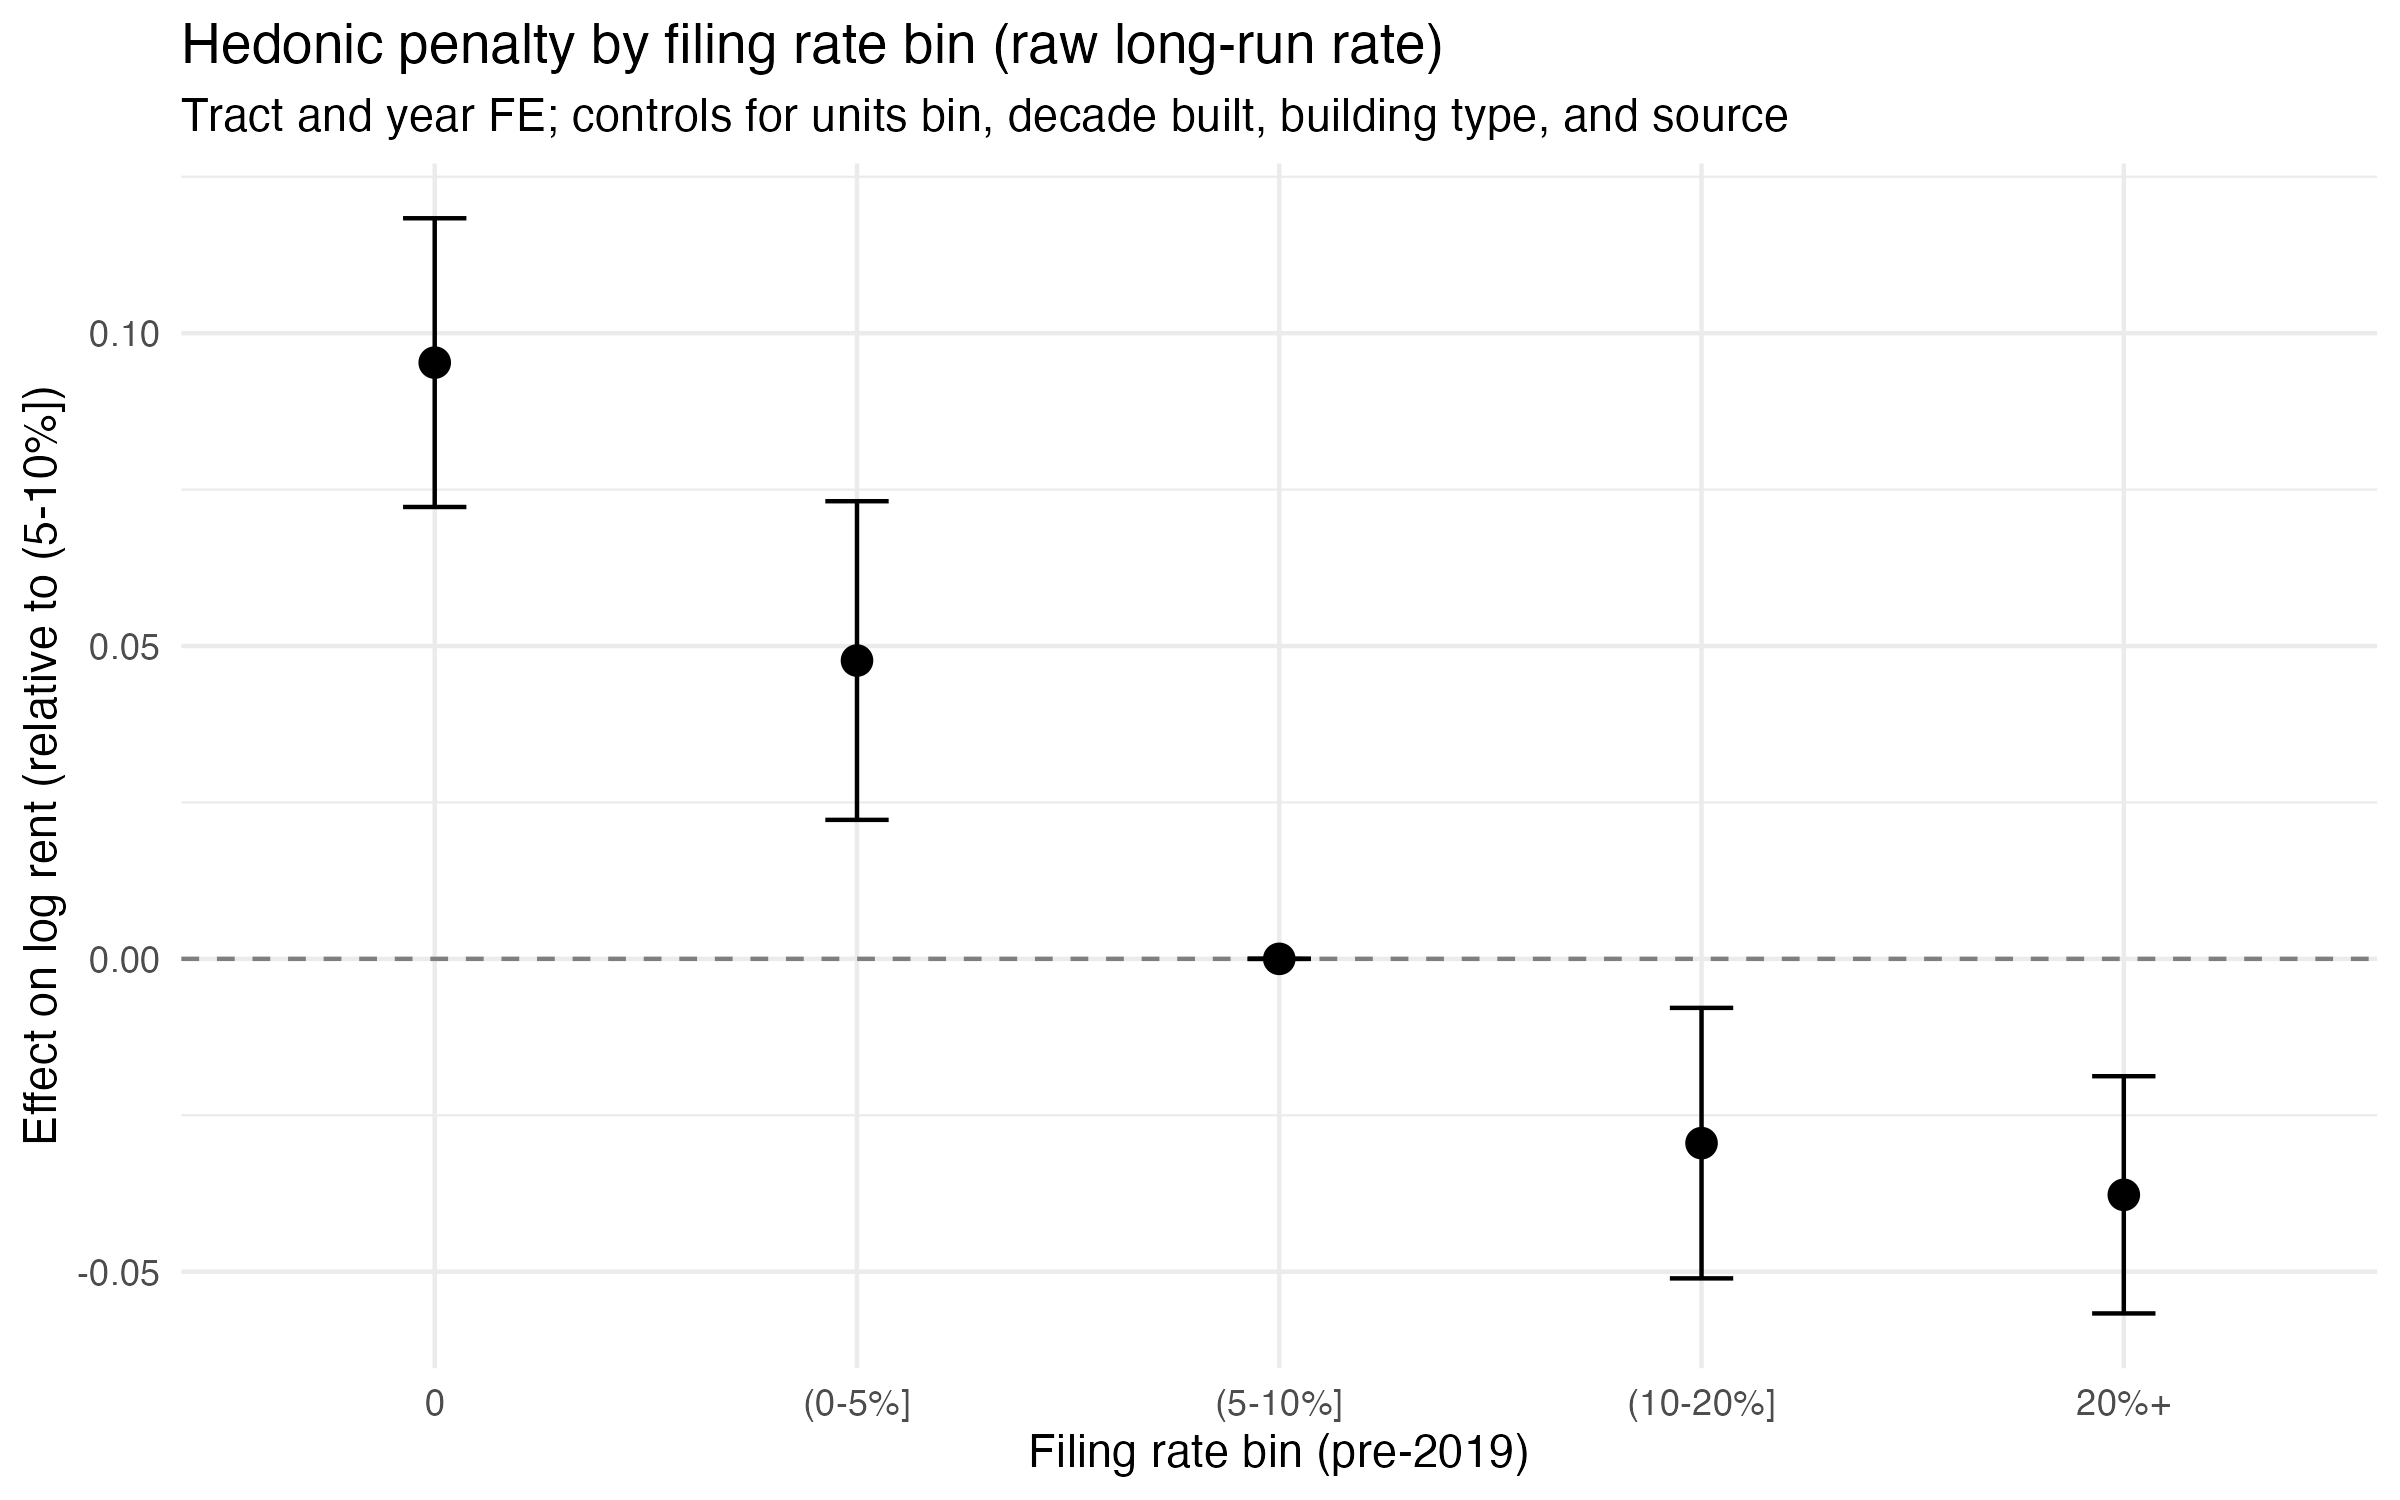
\includegraphics[width=0.95\linewidth,height=\textheight,keepaspectratio]{../output/price-regs/figs/coefplot_hedonic_filing_rate_longrun.png}

}

\caption{Hedonic rent penalty by raw filing rate bin (baseline
specification). Reference category: 5-10 percent filing rate bin. Tract
and year FE with building controls.}

\end{figure}%

\newpage

\section{Exploratory Diagnostics}\label{exploratory-diagnostics}

These plots residualize both rent and filing rate on the same controls
and fixed effects used in the hedonic regressions, then examine the
remaining relationship.

\subsection{Residual Variation in Raw Filing
Rate}\label{residual-variation-in-raw-filing-rate}

\begin{figure}[H]

{\centering 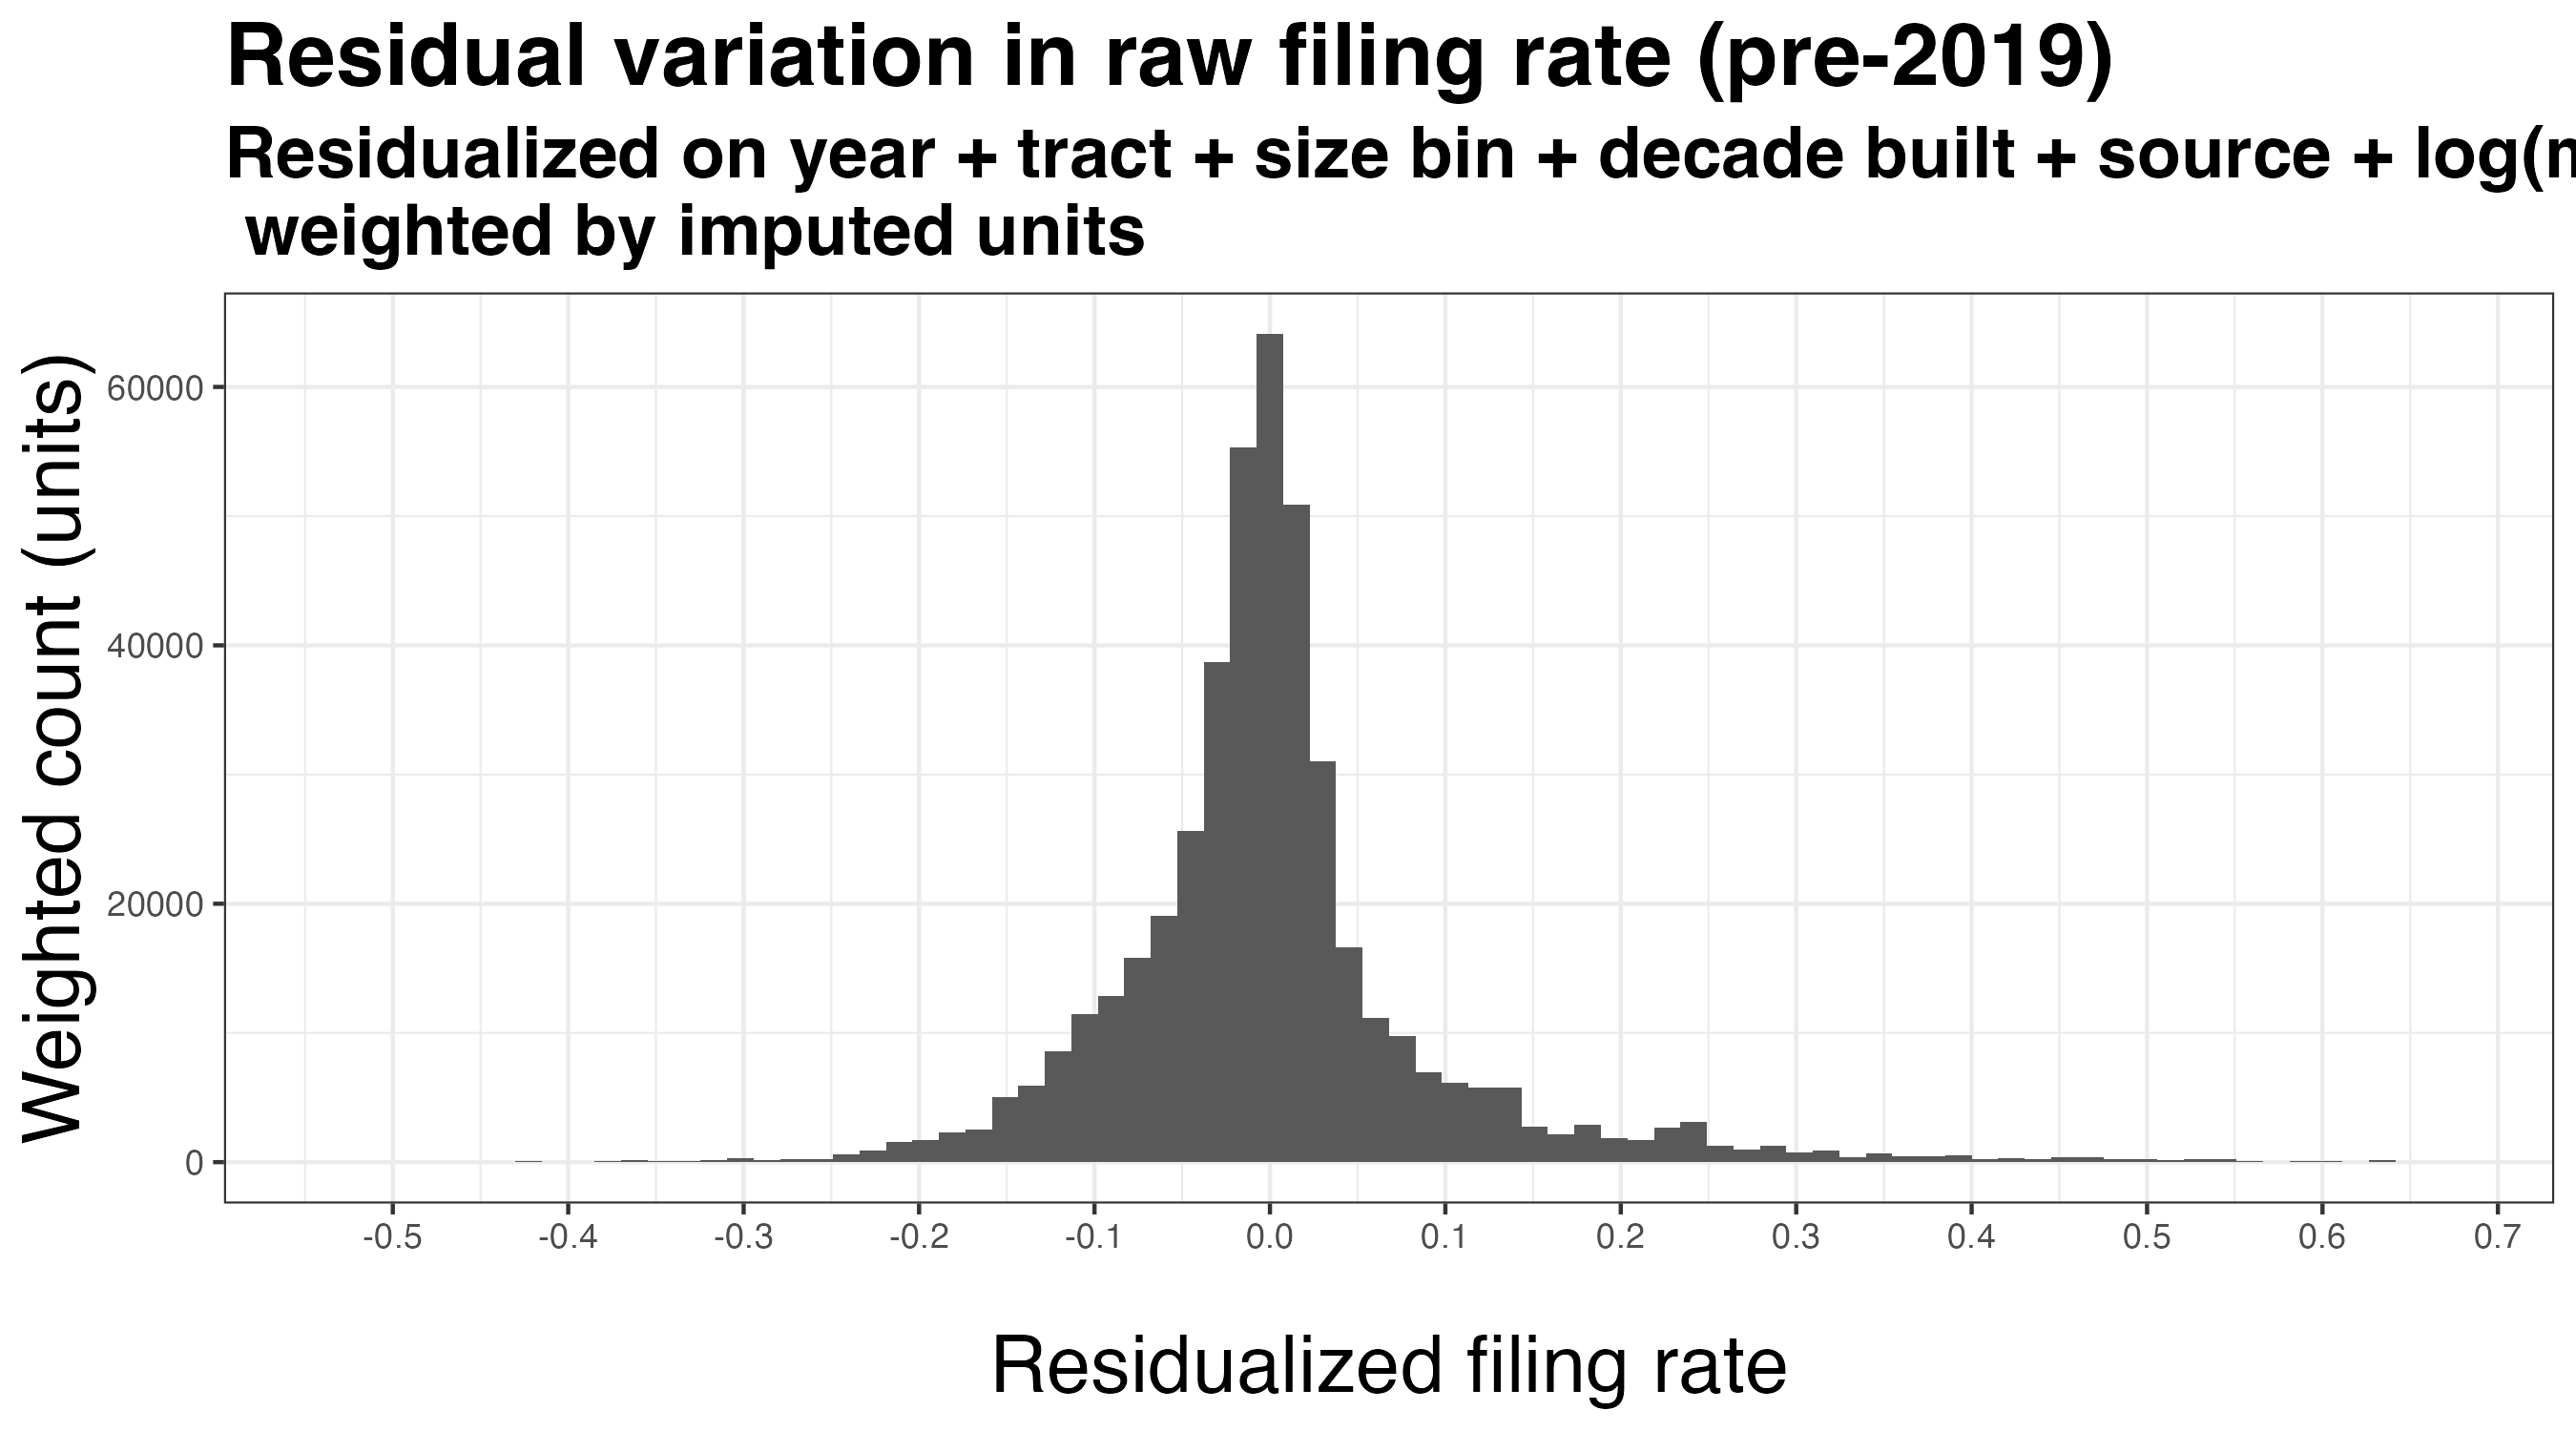
\includegraphics[width=0.95\linewidth,height=\textheight,keepaspectratio]{../output/price-regs/figs/resid_filing_rate_longrun_pre2019_hist.png}

}

\caption{Distribution of residualized raw filing rate (pre-2019).
Residualized on year + tract + building controls; weighted by total
units.}

\end{figure}%

\subsection{Residualized Rent vs Filing Rate: Bin
Scatter}\label{residualized-rent-vs-filing-rate-bin-scatter}

\begin{figure}[H]

{\centering 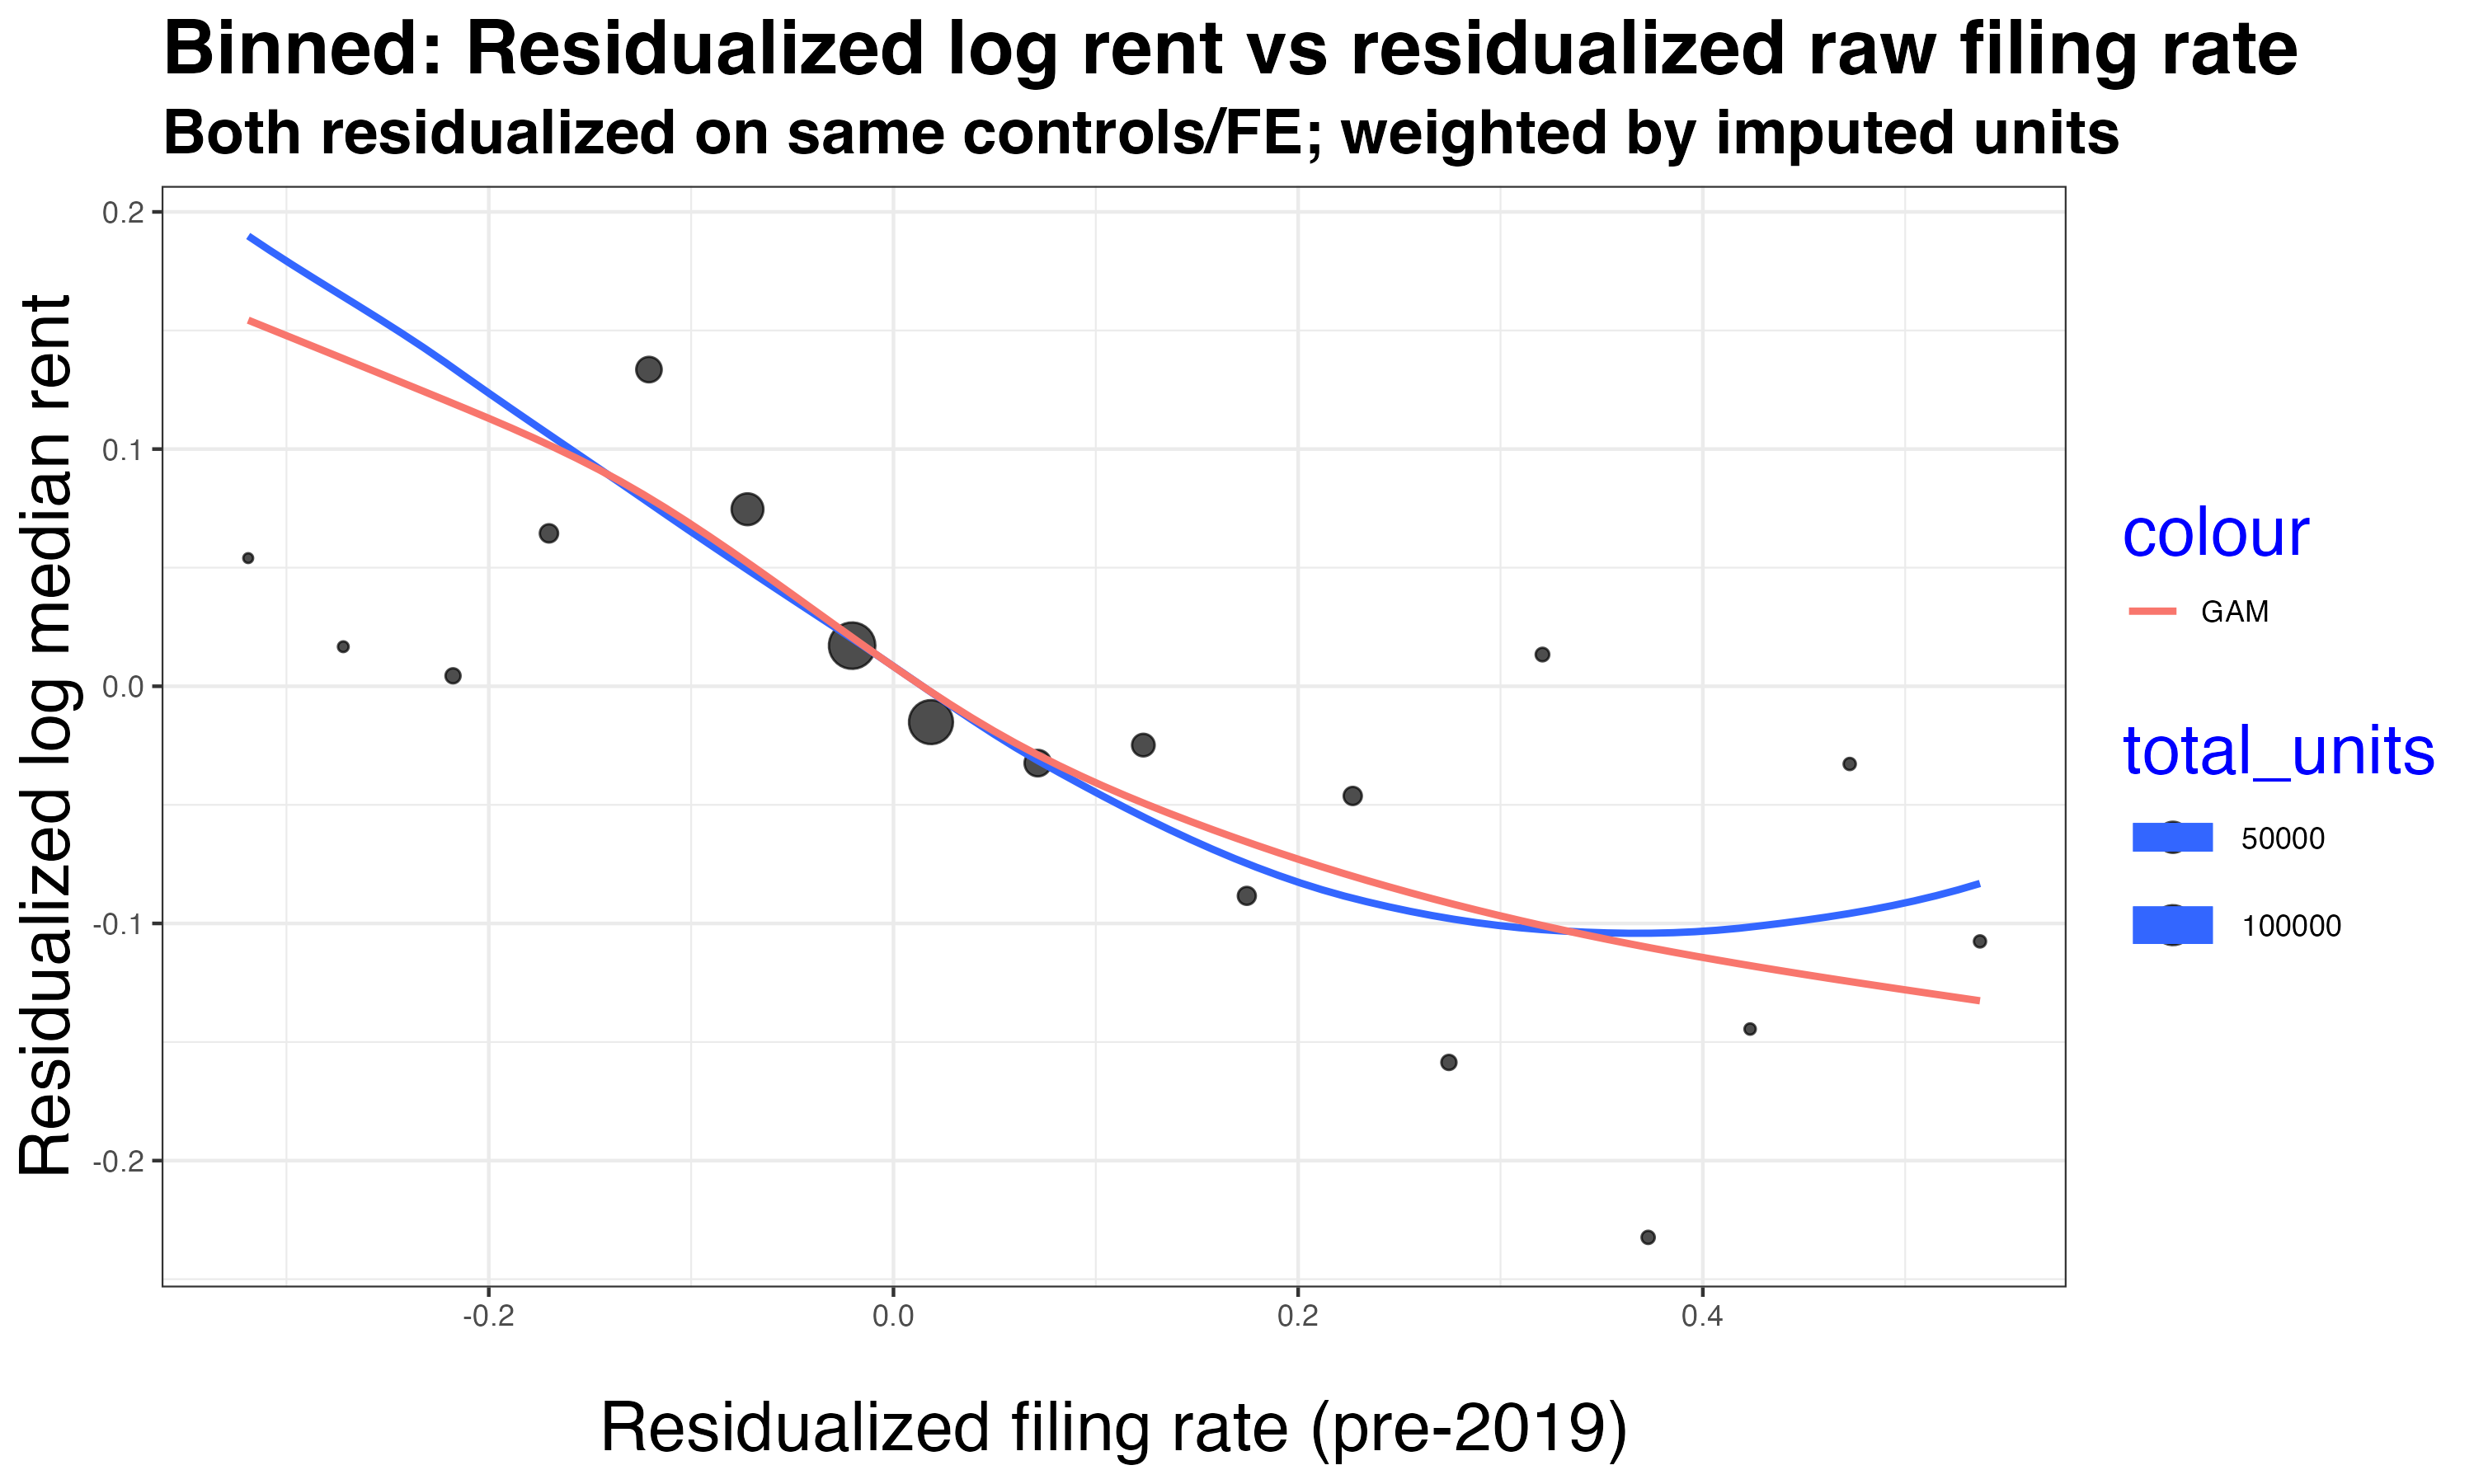
\includegraphics[width=0.95\linewidth,height=\textheight,keepaspectratio]{../output/price-regs/figs/binscatter_resid_rent_vs_filing_rate_longrun.png}

}

\caption{Binned scatter of residualized log rent vs residualized raw
filing rate. Both residualized on the same controls/FE; weighted by
total units.}

\end{figure}%

\subsection{Spline-Implied Stigma Curve
(Cubic)}\label{spline-implied-stigma-curve-cubic}

\begin{figure}[H]

{\centering 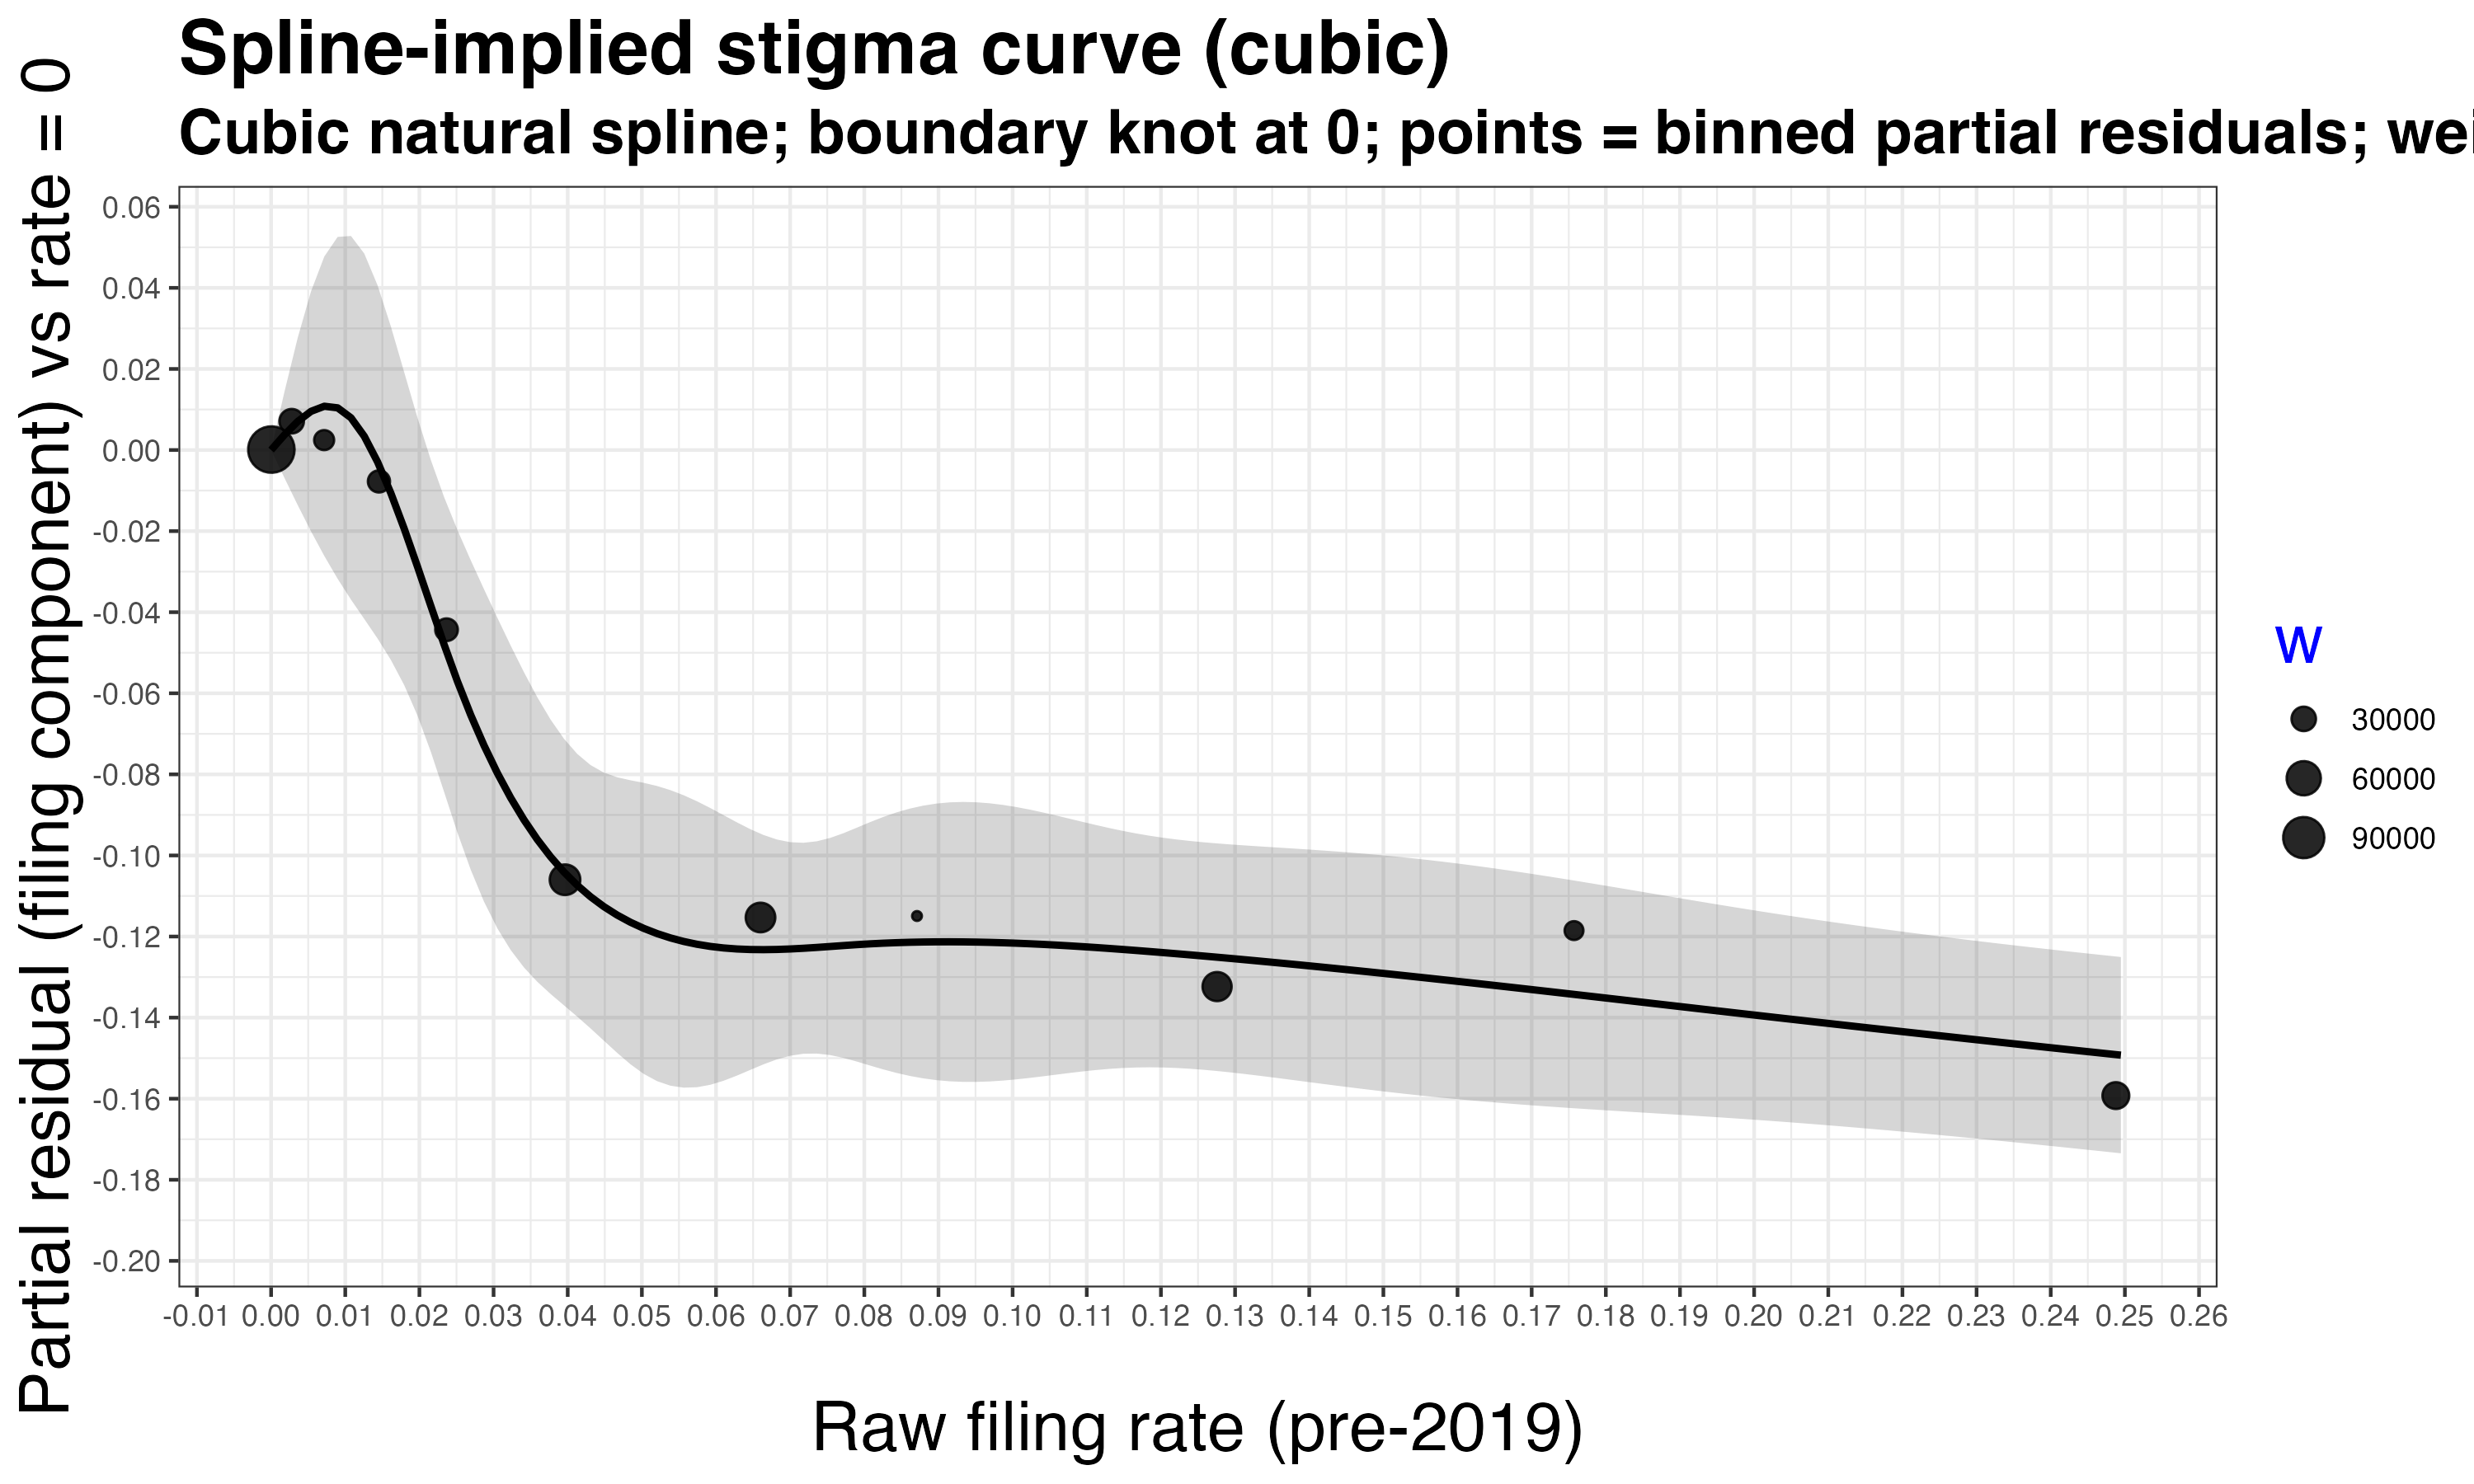
\includegraphics[width=1\linewidth,height=\textheight,keepaspectratio]{../output/price-regs/figs/spline_stigma_curve_raw.png}

}

\caption{Spline-implied stigma curve with partial-residual binned means.
The curve shows the fitted cubic natural spline component of log rent as
a function of raw filing rate (relative to never-filers), with 95\%
confidence band. Points are binned means of partial residuals.}

\end{figure}%

\subsection{Spline Robustness: Linear vs Quadratic vs
Cubic}\label{spline-robustness-linear-vs-quadratic-vs-cubic}

To assess sensitivity of the stigma curve shape to the smoothness
assumption, we estimate three spline specifications with identical knot
placement (concentrated at low filing rates: 1\%, 2.5\%, 5\%, 8\%, 12\%,
20\%):

\begin{itemize}
\tightlist
\item
  \textbf{Linear (degree 1):} Piecewise-linear with kinks at each knot.
  Imposes no curvature within segments; slope changes occur only at
  knots.
\item
  \textbf{Quadratic (degree 2):} Piecewise-quadratic; allows smooth
  curvature but constrains the second derivative to be
  piecewise-constant.
\item
  \textbf{Cubic (degree 3, natural spline):} Piecewise-cubic with
  natural boundary constraints (linear beyond boundary knots). Most
  flexible within the interior.
\end{itemize}

\begin{figure}[H]

{\centering 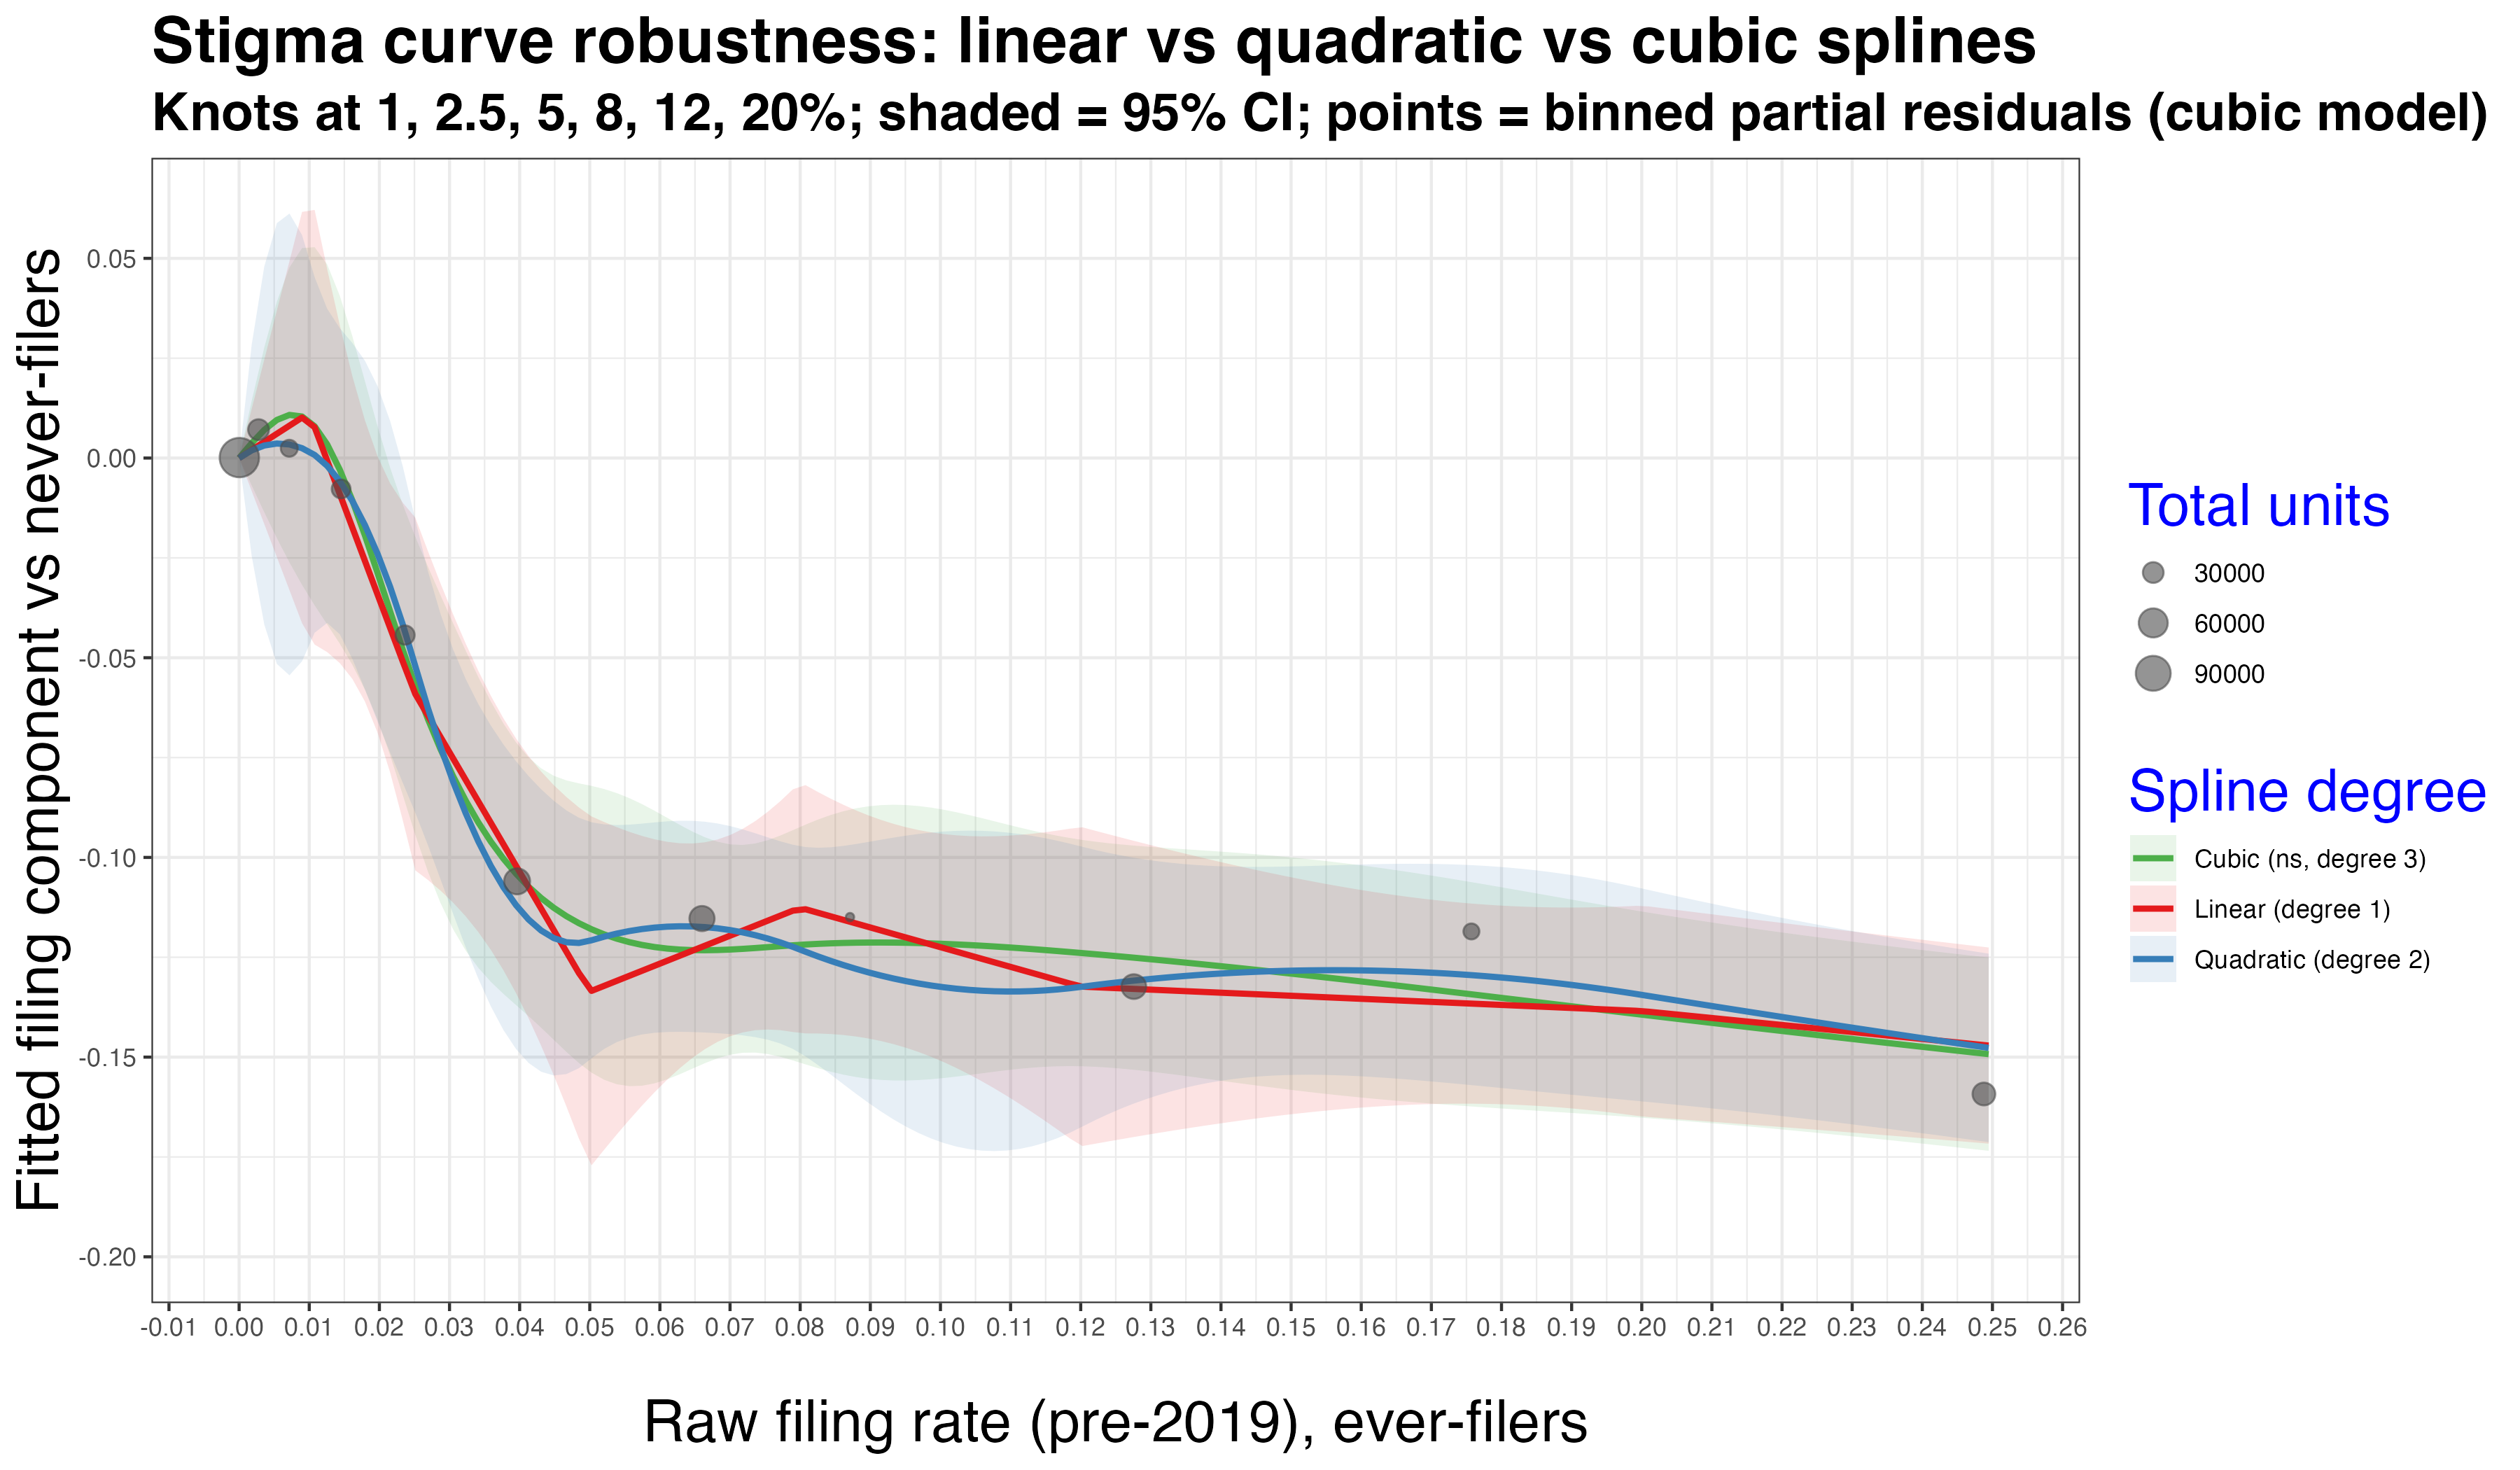
\includegraphics[width=1\linewidth,height=\textheight,keepaspectratio]{../output/price-regs/figs/spline_stigma_curve_comparison.png}

}

\caption{Comparison of stigma curves across spline degrees. All three
specifications use the same knots concentrated at low filing rates.
Shaded regions are 95\% confidence bands (delta method). Points are
binned partial residuals from the cubic model.}

\end{figure}%

\subsection{Hump Diagnostic: Never-Filer
Composition}\label{hump-diagnostic-never-filer-composition}

The spline curves show a hump near zero filing rate: buildings with very
low positive rates appear to have \emph{higher} rents than never-filers.
This reflects composition differences --- never-filers are 100\%
Altos-sourced (since eviction court records mechanically require a
filing), include 25\% single-family homes, and have a median of 1 unit.
The barely-ever-filers ((0, 1\%{]} bin) are large, high-quality
apartment complexes (median 46 units, 26\% quality-A).

To test whether the hump is a composition artifact, we re-estimate the
cubic spline under progressively richer controls:

\begin{enumerate}
\def\labelenumi{\arabic{enumi}.}
\tightlist
\item
  \textbf{Baseline} (no source FE --- as in the main spline)
\item
  \textbf{+ Source FE} (absorbs Altos vs eviction-court rent level
  differences)
\item
  \textbf{+ Source FE + panel tenure} (controls for years observed
  pre-2019)
\item
  \textbf{Multi-family only} (drops SFH, which are 25\% of never-filers)
\item
  \textbf{Multi-family + source + tenure} (all three adjustments)
\end{enumerate}

\begin{figure}[H]

{\centering 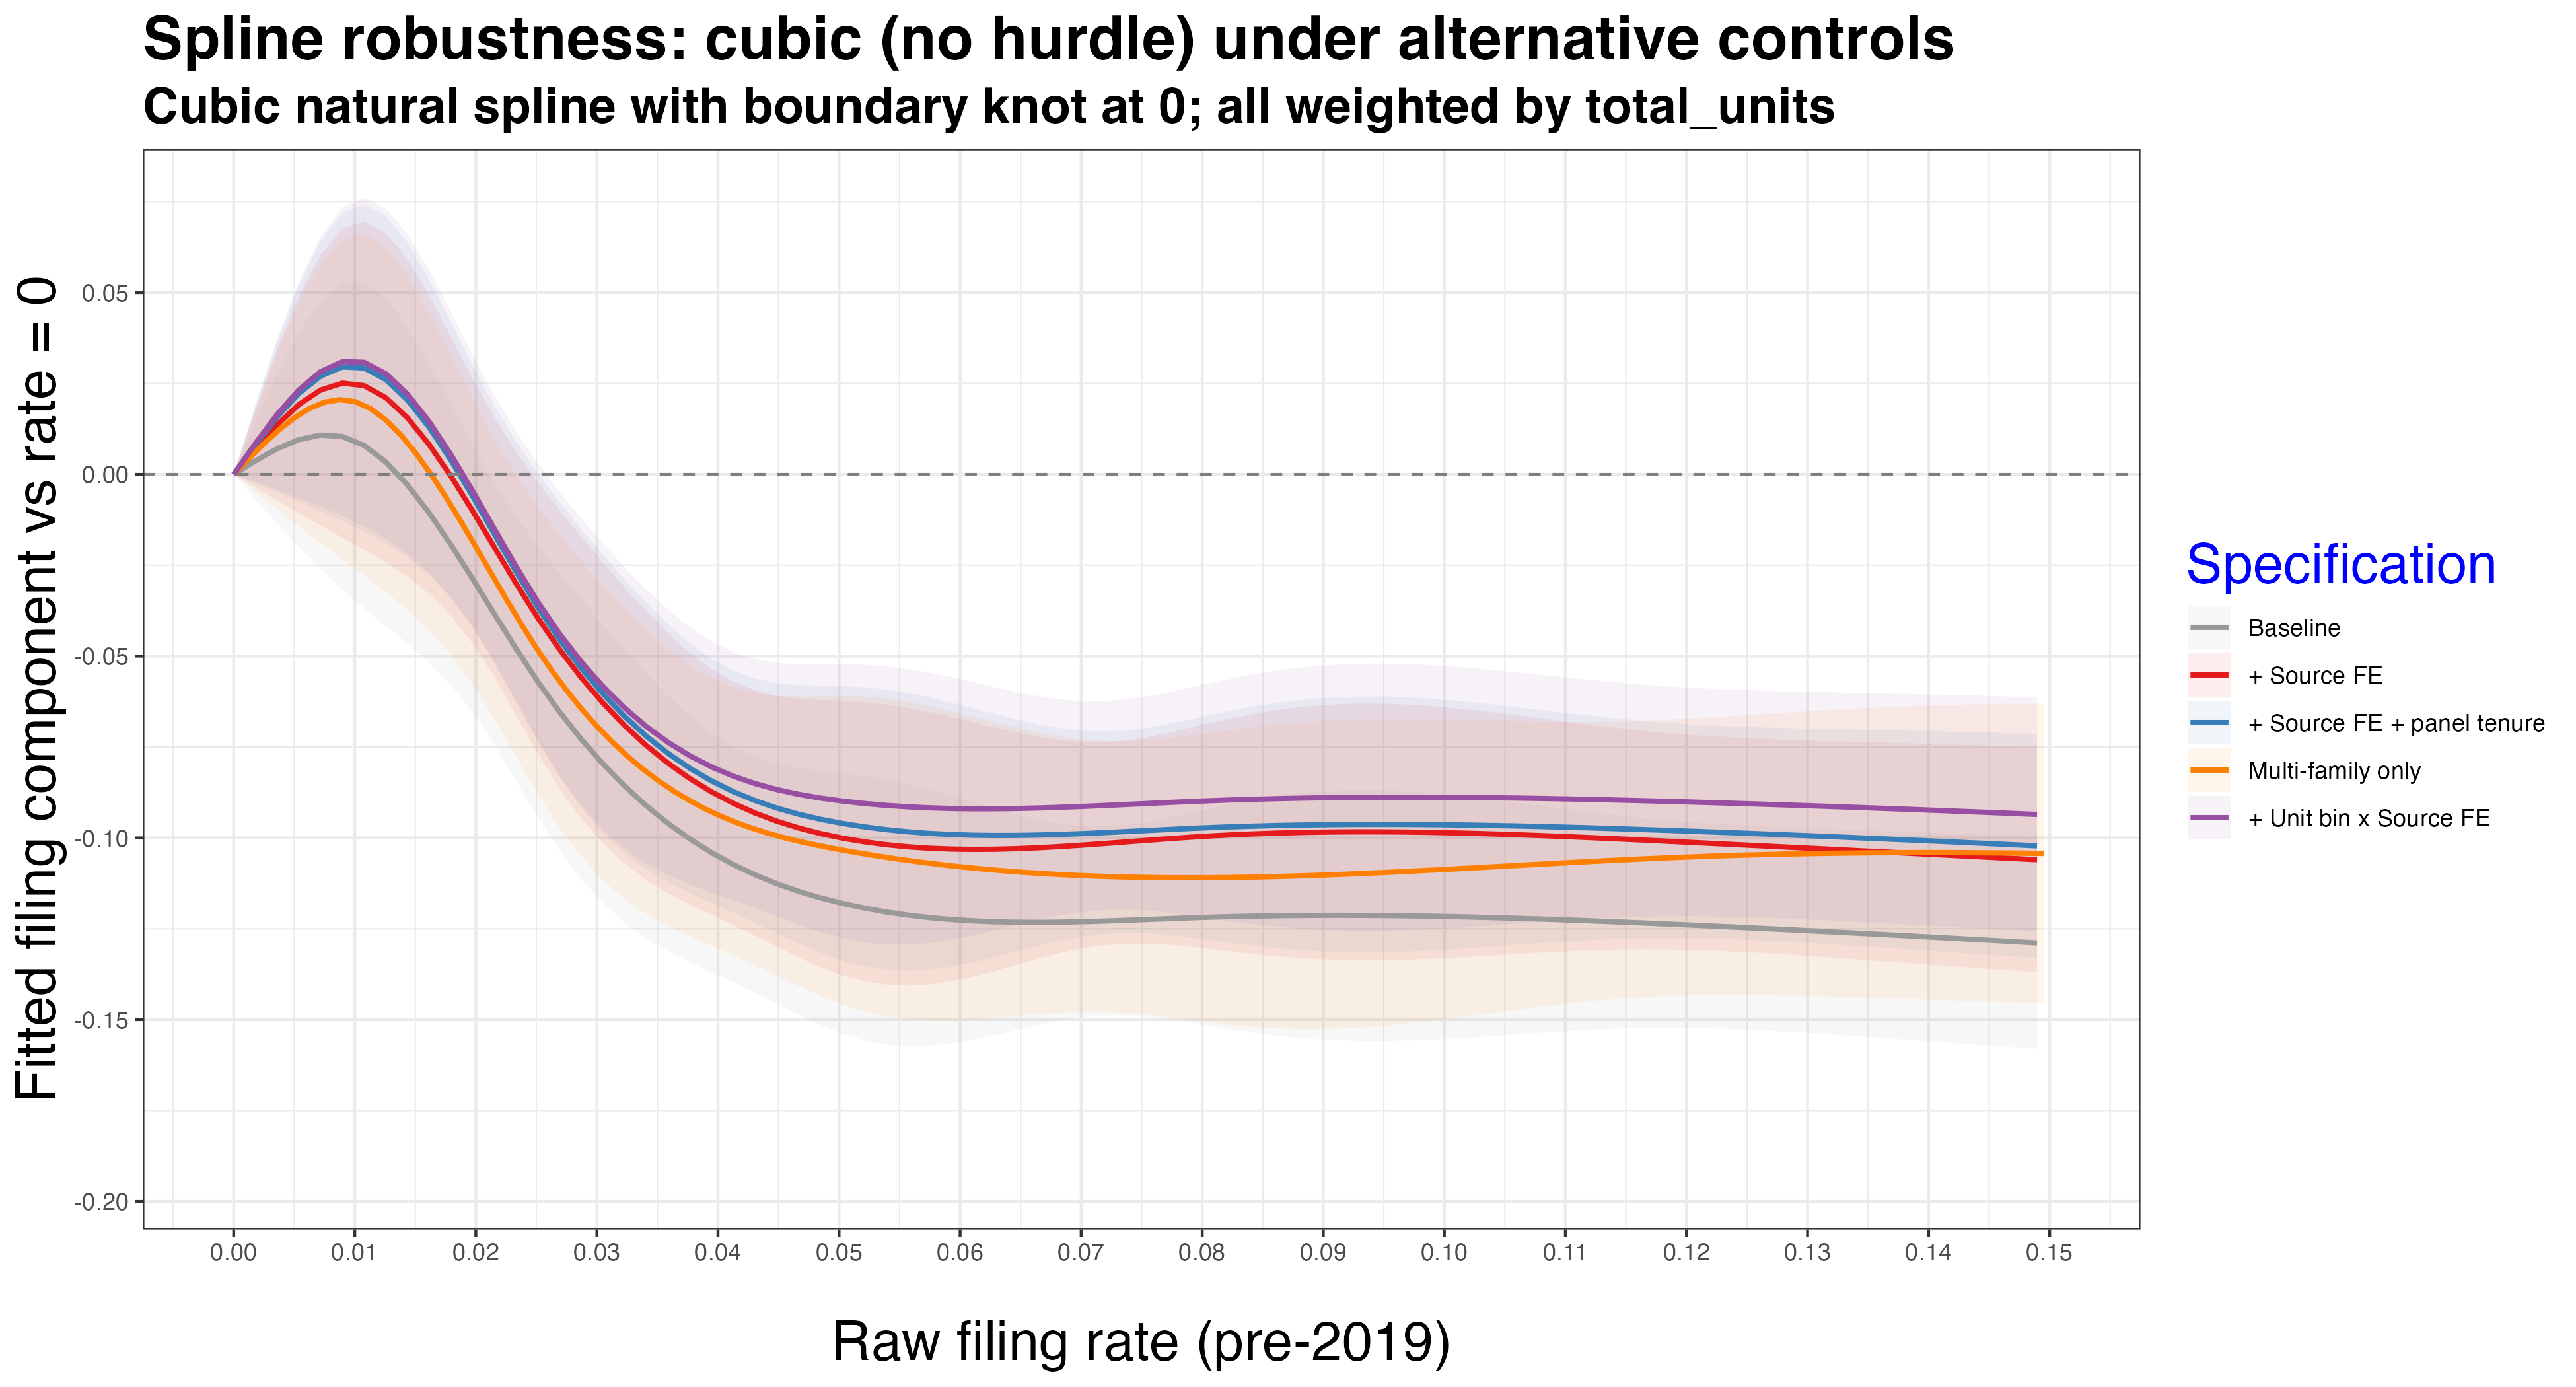
\includegraphics[width=1\linewidth,height=\textheight,keepaspectratio]{../output/price-regs/figs/spline_hump_diagnostic.png}

}

\caption{Hump diagnostic: cubic spline under alternative controls and
sample restrictions. Hump attenuates with source FE and disappears when
restricting to multi-family buildings.}

\end{figure}%

\newpage

\section{Interpretation}\label{interpretation}

The hedonic regressions estimate the \textbf{rent penalty} (or premium)
associated with eviction filing intensity, conditional on neighborhood
(tract FE) and building observables. Key quantities:

\begin{itemize}
\tightlist
\item
  \textbf{Binned model (Model 1):} The coefficient on the 20\%+ bin
  relative to (5--10\%{]} gives the rent differential for the
  highest-evicting buildings vs moderate-evicting buildings \emph{within
  the same tract and building type}.
\item
  \textbf{Continuous model (Model 2):} A one-unit increase in raw filing
  rate (e.g., from 0 to 1, which spans the entire range) is associated
  with a \(\beta\)-log-point change in rent. For typical variation (0 to
  0.20), multiply by 0.20.
\item
  \textbf{Tenant composition stability:} If adding tenant composition
  controls (Models 3--4) substantially attenuates the eviction intensity
  coefficients, it suggests the rent--eviction relationship partly
  reflects sorting by demographics. If coefficients are stable, the
  relationship is robust to observable tenant composition.
\item
  \textbf{Complaint \(\times\) high-eviction interaction (Model 5):}
  Tests whether buildings with both habitability complaints and high
  eviction rates have differentially lower rents, consistent with a
  ``stigma'' or quality channel.
\end{itemize}

\subsection{Comparison with EB
Estimates}\label{comparison-with-eb-estimates}

The raw long-run filing rate differs from the Empirical Bayes version in
\texttt{price-regs-eb.R}:

\begin{itemize}
\tightlist
\item
  \textbf{Raw rate:} Simple ratio of total filings to total units to
  years observed. Noisier for small buildings (few units, few years).
\item
  \textbf{EB rate:} Shrinks extreme raw rates toward a prior (city- or
  ZIP-level mean). More stable for buildings with thin data.
\end{itemize}

Both should produce qualitatively similar results for large,
well-observed buildings. Differences for small buildings reflect the EB
shrinkage pulling extreme rates toward the mean.




\end{document}
